\chapter{Métodos}

Neste capitulo percorremos as experiências realizadas. Estas foram feitas atraves do usos do programas criados para o efeito disponiveis no repositorio GitHub do \href{https://github.com/JotaFan/renewable-generation-into-reserve-markets}{projecto}.

\section{Benchmark}

Como modelo bencharmark iremos usar os atributos de alocação nos dados

TODO: explicar e adicionar imagens


\section{Modelos estatiscos  \label{se:dados_estudo}}

Antes de entrar para o densenvolvimento de modelos vamos usar metódos e modelos abertos para usar comparativamente.
Para as equações apresentadas temos que \textit{$Y_t$} é a variavel alvo, no tempo \textit{t}

\subsection{AR}

AR eé blabla

\begin{equation} \label{eq:AR} Y_t = c + \phi_1 Y_{t-1} + \phi_2 Y_{t-2} + \dots + \phi_p Y_{t-p} + \varepsilon_t \end{equation}

\begin{figure}[H]
    \centering
    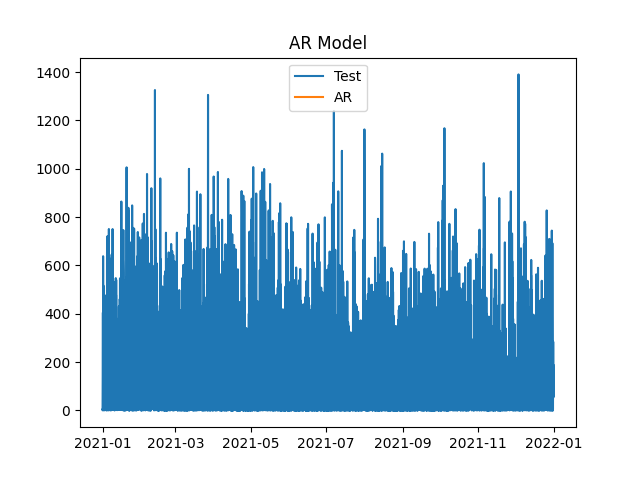
\includegraphics[width=0.8\textwidth]{../plots/AR_model.png}
    \caption{Previsões 2022 com model AR}
    \label{fig:AR_model}
\end{figure}
  



\subsection{MA}

AR eé blabla

\begin{equation} \label{eq:MA} 
    Y_t = c + \theta_1 \varepsilon_{t-1} + \theta_2 \varepsilon_{t-2} + \dots + \theta_q \varepsilon_{t-q} + \varepsilon_t 
\end{equation}

\begin{figure}[H]
    \centering
    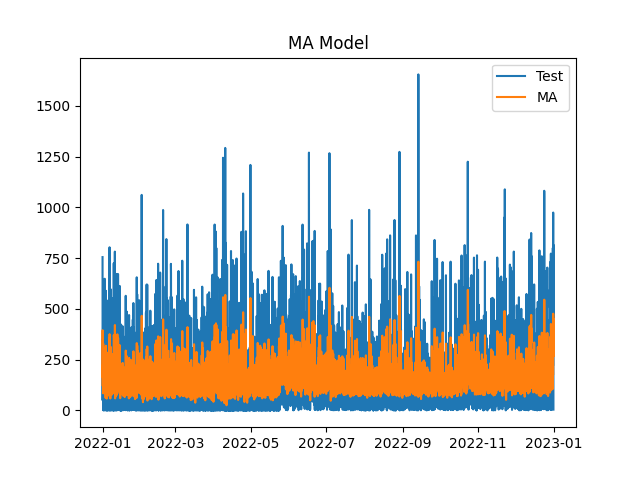
\includegraphics[width=0.8\textwidth]{../plots/MA_model.png}
    \caption{Previsões 2022 com model MA}
    \label{fig:MA_model}
\end{figure}
  
\subsection{ARMA}

AR eé blabla

\begin{equation} \label{eq:ARMA}  Y_t = c + \phi_1 Y_{t-1} + \phi_2 Y_{t-2} + \dots + \phi_p Y_{t-p} + \theta_1 \varepsilon_{t-1} + \theta_2 \varepsilon_{t-2} + \dots + \theta_q \varepsilon_{t-q} + \varepsilon_t  \end{equation}

\begin{figure}[H]
    \centering
    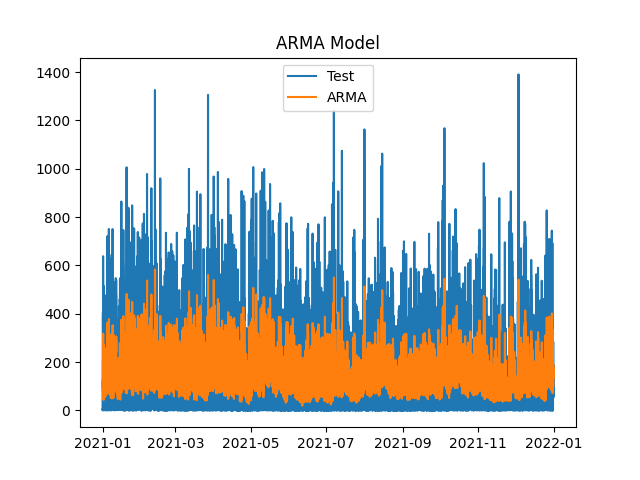
\includegraphics[width=0.8\textwidth]{../plots/ARMA_model.png}
    \caption{Previsões 2022 com model ARMA}
    \label{fig:ARMA_model}
\end{figure}

\subsection{ARIMA}

AR eé blabla

\begin{equation} \label{eq:ARIMA} Y't = c + \phi_1 Y'{t-1} + \phi_2 Y'{t-2} + \dots + \phi_p Y'{t-p} + \theta_1 \varepsilon_{t-1} + \theta_2 \varepsilon_{t-2} + \dots + \theta_q \varepsilon_{t-q} + \varepsilon_t \end{equation}

\begin{figure}[H]
    \centering
    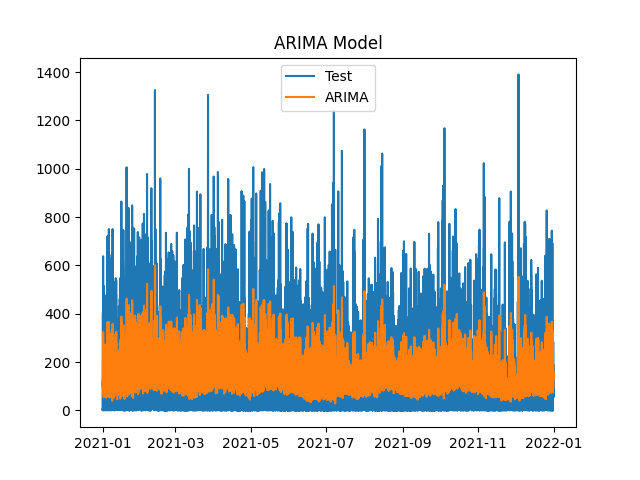
\includegraphics[width=0.8\textwidth]{../plots/ARIMA_model.png}
    \caption{Previsões 2022 com model ARIMA}
    \label{fig:ARIMA_model}
\end{figure}

\subsection{SARIMA}

AR eé blabla

\begin{equation} \label{eq:SARIMA} Y_t = c + \phi_1 Y_{t-1} + \phi_2 Y_{t-2} + \dots + \phi_p Y_{t-p} + \theta_1 \varepsilon_{t-1} + \theta_2 \varepsilon_{t-2} + \dots + \theta_q \varepsilon_{t-q} + \varepsilon_t \end{equation}

\begin{figure}[H]
    \centering
    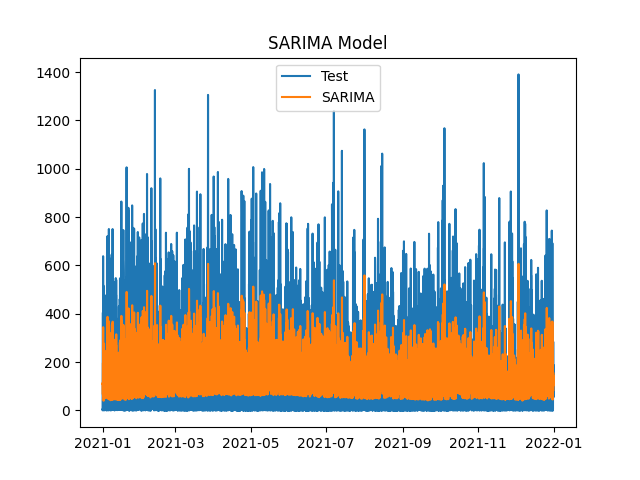
\includegraphics[width=0.8\textwidth]{../plots/SARIMA_model.png}
    \caption{Previsões 2022 com model SARIMA}
    \label{fig:SARIMA_model}
\end{figure}


TODO: criar csv com resultados disto

\section{Forecat  \label{se:dados_estudo}}

Com o propósito de desenvolver este estudo, e deixar ferramentas para a replicação do mesmo, foi criado uma biblioteca em python para desenhar as arquitecturas em estudo.


\subsection{Construtor de modelos}


\subsection{subsubsection Gerador de dados (depth 2)}
distribuiçao

clustering


\section{Treino e Resultados  \label{se:dados_estudo}}

Realizaram-se várias experiências, onde em cada um se ia elimando alguns dos objectos em estudo.
Em casa experiências toda a parametrização era igual, à excepção do objecto de estudo.

\subsection{Arquiteturas e numeros de epocas}

Nesta experiência foi testado o resultado das várias arquiteturas em estudo, como tambem o impacto do numero de epocas na qualidade dos modelos-
As arquitecturas estudadas foram:

\begin{itemize}
    \item[--] VanillaDense
    \item[--] VanillaCNN
    \item[--] VanillaLSTM
    \item[--] StackedCNN
    \item[--] StackedLSTM
    \item[--] EncoderDecoder
    \item[--] UNET
\end{itemize}

O modelos foram treinados em 200 epocas, sendo que foram salvos a cada 15 epocas, de forma conseguirmos perceber os contextos nos saltos de epocas.

As parametrizações usadas:
\begin{itemize}
    \item[--] loss : mean squared error
    \item[--] Metodo activação no meio : relu
    \item[--] Metodo activação no fim : relu
    \item[--] optimizador : Adam
    \item[--] Janela temporal em X : 168 horas (1 semana)
    \item[--] Janela temporal em Y : 24 horas (1 semana)
    \item[--] Fracção de treino : 95%  
\end{itemize}

\subsection{Funções de Perda (Loss)}

TODO: o que é a loss function?

Esta experiência consiste em rever que função de perda é melhor aplicavel ao problema. Sendo um problema de regressao linear, de valores bastante oscilatórios e com uma distribuição exponencial, temos algumas loss functions que já são reconhecidas para o problema.

\begin{itemize}
    \item[--] mean absolute error
    \item[--] mean squared error    
    \item[--] loss : mean absolute error

\end{itemize}



\subsection{subsubsection Gerador de dados (depth 2)}
distribuiçao

clustering


\section{Considerações adicionais  \label{se:dados_plus}}

Foram realizados testes adicionais que não obtiveram resultados passivos de boa interpretação, e foram imediatamente descartados, como:

\begin{itemize}
    \item[--] Janela temporal em X : 96, 48, 24
    \item[--] optimizador : todos os optimizadores disponiveis na biblioteca keras
    \item[--] loss : todas as outra loss functions de regressão disponiveis.
    \item[--] epocas : influência do numero de epocas nos modelos, foram treinados até 20000 epocas alguns modelos mas à medida que a perda ia estagnando na assintomta, o modelo ia apenas piorando.
\end{itemize}

